\documentclass[12pt]{article}

% Set the page to be letter paper and have small margins
\usepackage{geometry}
\geometry{letterpaper, left=15mm, right=15mm, top=15mm, bottom=20mm}

% LuaLaTeX font setup
\usepackage{fontspec}
\usepackage{unicode-math}

% Text font
\setmainfont{DejaVu Serif}

% Math font
\setmathfont{STIX Two Math}

\allowdisplaybreaks[1]

\usepackage{standalone}
\usepackage{parskip}
\usepackage{amsmath}
\usepackage{amsthm}
\usepackage{multicol}
\usepackage{graphicx}
\usepackage{pgfplots}
\pgfplotsset{compat=1.18}
\usepackage{cancel}
\usepackage{xcolor}
\usepackage[utf8]{inputenc}
\usepackage{float}
\usepackage{graphicx}
\usepackage{pdfpages}
\usepackage{booktabs}

% \usepackage{hyperref}
\usepackage{cleveref}


\usepackage{titlesec}
\titleformat{\section}{\normalfont\normalsize\bfseries}{\thesection.}{1em}{}
\titleformat{\subsection}{\normalfont\normalsize\bfseries\itshape}{\thesubsection}{1em}{}

\usepackage{enumitem}
\setlist[enumerate, 1]{label=\textbf{\arabic*}.}
\setlist[enumerate, 2]{label=\textbf{\alph*}.}

% \usepackage[style=ieee]{biblatex}
% \addbibresource{src/refs.bib}

\makeatletter
\newcommand{\course}[1]{\def\@course{#1}}

\renewcommand{\maketitle}{
    \noindent
    \@author \hfill \@course \newline
    \@date
    \begin{center}
        \large\textbf{\@title}
    \end{center}
    \bigskip
}

\author{Jeffrey Morris}
\course{MATH 4306-010}
\date{\today}


\begin{document}
\begin{align*}
    f(-x) & =\left|\sin(-x)\right|            \\
          & =\left|-\sin(x)\right|            \\
          & =\left|sin(x)\right| = f(x)       \\
          & \Rightarrow f(x) \text{ is even.}
\end{align*}
\begin{align*}
    a_0= & \frac{1}{2\pi}\int_{-\pi}^{\pi}f(x)\,dx      \\
    a_0= & \frac{1}{\pi}\int_{0}^{\pi}\sin(x)\,dx       \\
    a_0= & \frac{1}{\pi}\left[-\cos(x)\right]_{0}^{\pi} \\
    a_0= & \frac{1}{\pi}\left[-\cos(\pi)+\cos(0)\right] \\
    a_0= & \frac{1}{\pi}\cdot 2                         \\
    a_0= & \boxed{\frac{2}{\pi}}
\end{align*}
\begin{align*}
    a_n= & \frac{1}{\pi}\int_{-\pi}^{\pi}f(x)\cos(nx)\,dx                                                                                                                                     \\
    a_n= & \frac{2}{\pi}\int_{0}^{\pi}\sin(x)\cos(nx)\,dx                                                                                                                                     \\
    a_n= & \frac{2}{\pi}\int_{0}^{\pi}\frac{1}{2}\left[\sin(x+nx)+sin(x-nx)\right]\,dx                                                                                                        \\
    a_n= & \frac{1}{\pi}\sin\left((n+1)\cdot x\right)-\sin\left((n-1)\cdot x\right)\,dx                                                                                                       \\
    a_n= & \frac{1}{\pi} \left[ \frac{-\cos\left((n+1) \cdot x\right)}{n+1} + \frac{\cos\left((n-1)\cdot x\right)}{n-1} \right]_{0}^{\pi}                                                     \\
    a_n= & \frac{1}{\pi} \left[ \left( \frac{-\cos\left((n+1) \cdot \pi\right)}{n+1} + \frac{\cos\left((n-1)\cdot\pi\right)}{n-1}\right) - \left(\frac{-1}{n+1} + \frac{1}{n+1}\right)\right] \\
    a_n= & \frac{1}{\pi} \left[ \frac{(-1)^n}{n+1} + \frac{-(-1)^n}{n-1} + \frac{1}{n+1} + \frac{-1}{n-1}\right]                                                                              \\
    a_n= & \frac{1}{\pi} \left[ \frac{1+(-1)^n}{n+1} - \frac{1+(-1)^n}{n-1} \right]                                                                                                           \\
    a_n= & \frac{1+(-1)^n}{\pi} \left[ \frac{-2}{n^2-1} \right]                                                                                                                               \\
    a_n= &
    \boxed{
        \begin{cases}
            0,                                          & \text{if $n$ is odd}  \\
            \frac{-4}{\left( n^2 - 1 \right)\cdot \pi}, & \text{if $n$ is even}
        \end{cases}
    }
\end{align*}
\begin{gather*}
    b_n=\frac{1}{\pi}\int_{-\pi}^{\pi}f(x)\sin(nx)\,dx \\
    \text{Since $f(x)$ is even, $b_n=\boxed{0}$ }
\end{gather*}
\begin{center}
    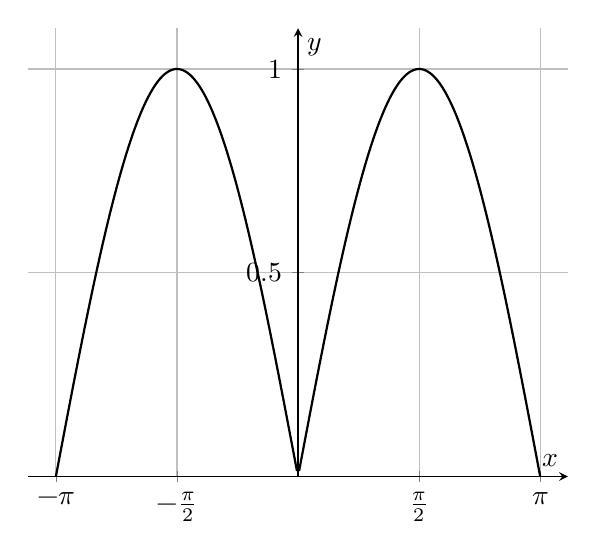
\begin{tikzpicture}
        \begin{axis}[
                axis lines=middle,
                grid=both,
                xmin=-3.5, xmax=3.5,
                ymin=0, ymax=1.1,
                xtick={-pi,-pi/2,0,pi/2,pi},
                xticklabels={$-\pi$,$-\frac{\pi}{2}$,$0$,$\frac{\pi}{2}$,$\pi$},
                ytick={0, 0.5, 1},
                xlabel={$x$}, ylabel={$y$},
                samples=200,
                domain=-pi:pi,
            ]
            \addplot[thick]{abs(sin(deg(x)))};
        \end{axis}
    \end{tikzpicture}
\end{center}
\end{document}